\documentclass{article}
\usepackage[paperwidth=188mm,paperheight=172mm,margin=4mm]{geometry}
\usepackage{graphicx}
\usepackage{tikz}
\usetikzlibrary{arrows.meta,positioning,shapes.geometric,fit,backgrounds,calc}
\pagestyle{empty}

\begin{document}
\noindent\resizebox{\textwidth}{!}{%
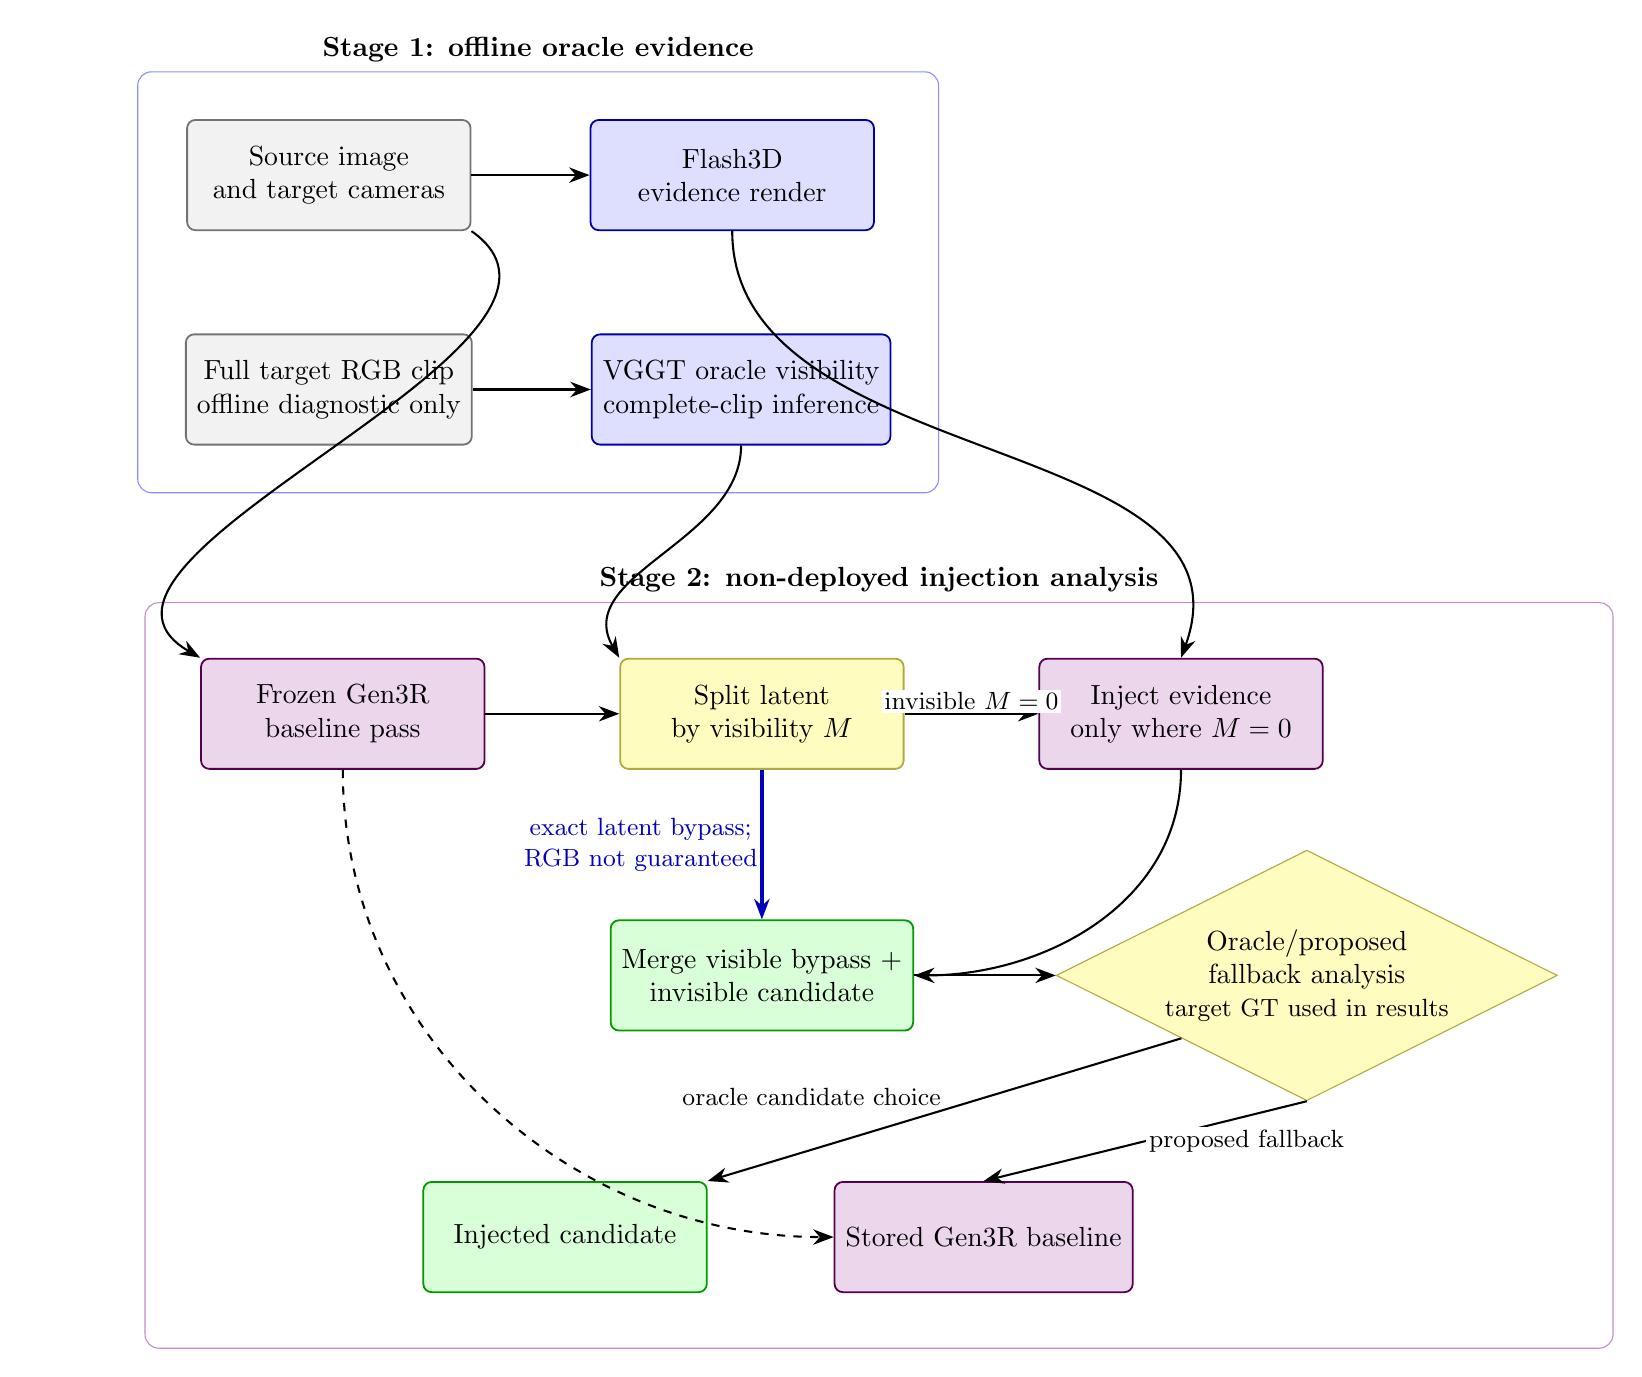
\begin{tikzpicture}[
  font=\normalsize,
  >={Stealth[length=2.6mm]},
  box/.style={rounded corners=3pt,draw,align=center,minimum height=14mm,minimum width=36mm,inner sep=4pt,line width=0.65pt},
  input/.style={box,fill=black!5,draw=black!55},
  geo/.style={box,fill=blue!13,draw=blue!65!black},
  gen/.style={box,fill=violet!16,draw=violet!65!black},
  mask/.style={box,fill=yellow!25,draw=yellow!65!black},
  output/.style={box,fill=green!15,draw=green!60!black},
  policy/.style={diamond,aspect=2.0,draw=yellow!65!black,fill=yellow!25,align=center,inner sep=2pt},
  flow/.style={->,line width=0.75pt},
  bypass/.style={->,line width=1.2pt,blue!75!black},
  note/.style={font=\small,align=center,fill=white,inner sep=1pt},
]

\node[input] (source) {Source image\\and target cameras};
\node[input,below=13mm of source] (clip) {Full target RGB clip\\offline diagnostic only};
\node[geo,right=15mm of source] (f3d) {Flash3D\\evidence render};
\node[geo,right=15mm of clip] (vggt) {VGGT oracle visibility\\complete-clip inference};
\node[fit=(source)(clip)(f3d)(vggt),draw=blue!45,rounded corners=5pt,inner sep=6mm,label={[font=\bfseries]above:Stage 1: offline oracle evidence}] (stage1) {};

\node[gen,below=28mm of stage1.south west,anchor=west,xshift=8mm] (base) {Frozen Gen3R\\baseline pass};
\node[mask,right=17mm of base] (split) {Split latent\\by visibility $M$};
\node[gen,right=17mm of split] (inject) {Inject evidence\\only where $M=0$};
\node[output,below=19mm of split] (merge) {Merge visible bypass +\\invisible candidate};
\node[policy,right=18mm of merge] (policy) {Oracle/proposed\\fallback analysis\\\small target GT used in results};
\node[output,below=19mm of merge,xshift=-25mm] (candidate) {Injected candidate};
\node[gen,right=16mm of candidate] (fallback) {Stored Gen3R baseline};
\node[fit=(base)(split)(inject)(merge)(policy)(candidate)(fallback),draw=violet!45,rounded corners=5pt,inner sep=7mm,label={[font=\bfseries]above:Stage 2: non-deployed injection analysis}] (stage2) {};

\draw[flow] (source) -- (f3d);
\draw[flow] (clip) -- (vggt);
\draw[flow] (source.south east) to[out=-35,in=150] (base.north west);
\draw[flow] (f3d.south) to[out=-90,in=70] (inject.north);
\draw[flow] (vggt.south) to[out=-90,in=120] (split.north west);
\draw[flow] (base) -- (split);
\draw[flow] (split) -- node[above,note]{invisible $M=0$} (inject);
\draw[flow] (inject.south) to[out=-90,in=0] (merge.east);
\draw[bypass] (split.south) -- node[left,note,text=blue!75!black]{exact latent bypass;\\RGB not guaranteed} (merge.north);
\draw[flow] (merge) -- (policy);
\draw[flow] (policy.south west) -- node[above left,note]{oracle candidate choice} (candidate.north east);
\draw[flow] (policy.south) -- node[right,note]{proposed fallback} (fallback.north);
\draw[flow,dashed] (base.south) to[out=-90,in=180] (fallback.west);
\end{tikzpicture}%
}
\end{document}
